
Our experiments consist of flying orbit trajectories, seen in Fig. 1., around a fixed point of interest. They are parameterized by the radius of the orbit, altitude, and the target linear velocity.  Each of these parameters is varied independently in our experiments with linear velocities: hover, 2, 4, 6, or 8 m/s; altitudes: 20, 25, or 30 m; and orbit radius: 25 or 50 m. 

The set of target linear velocities was chosen because we want to characterize how each terms' contribution in \eqref{powConsumed} vary with $v_\infty$. By tracking a variety of $v_g$ while orbiting, the quadrotor experiences an even larger range of $v_\infty$. The lower and upper bound were chosen because hovering is still one of the most common modes for a quadrotor and 8 m/s is approaching the dynamic limits of most commercially available platforms.

Similarly, the set of altitudes was chosen to verify our flights were conducted high enough to avoid viscous effects from the ground. Otherwise, our planar wind field assumption would be severely inaccurate. The lower bound of this set was a safety measure to ensure the quadrotor avoided standing structures at the airfield by at least 5 m.

Lastly, we chose to fly at two different orbit radii because $\phi$ is smaller at larger orbits, improving our approximations of $\alpha$ in \eqref{powConsumed}. 25 and 50 m were chosen because smaller radii make it dynamically challenging to fly at high linear velocities, whereas larger radii begin to encroach on the airfield's boundaries.  

%We chose orbit missions as our test case for several reasons: 
%\begin{enumerate}
%	\item Orbits provide a sweeping range of $\alpha$ and $v_\infty$
%	\item They are easily parameterized relative to other trajectory types
%	\item Their repetitive nature allows the use of statistical tools 
%	\item It is a typical flight mission for a quadrotor in practice
%\end{enumerate}

All our flights were conducted with a DJI M100 with Intel NUC7i7 onboard to handle high level control, communication with ground station, and some data logging. The majority of flight data comes from the onboard DJI flight log. The Matlab scripts and functions necessary to repeat our analysis can be found on our git repo. Parameters determined for our platform:
\begin{align*}
	m &= 3.29 \text{ kg} \\
	r &= 17.2 \text{ cm} \\
	\mu_1 &= 0.182 \\
	\mu_2 &= -0.023 \\
	\mu_3 &= 0.004 \\
	\kappa_1 &= 0.275 
\end{align*}
Where $\kappa_1$ was found following \cite{liu2017power}, and our determination of $\mu_1$, $\mu_2$, and $\mu_3$ is described in \ref{sec:Dynamics} .


%\begin{figure}[htbp]
%	\centering
%	\label{fig:exp6}
%	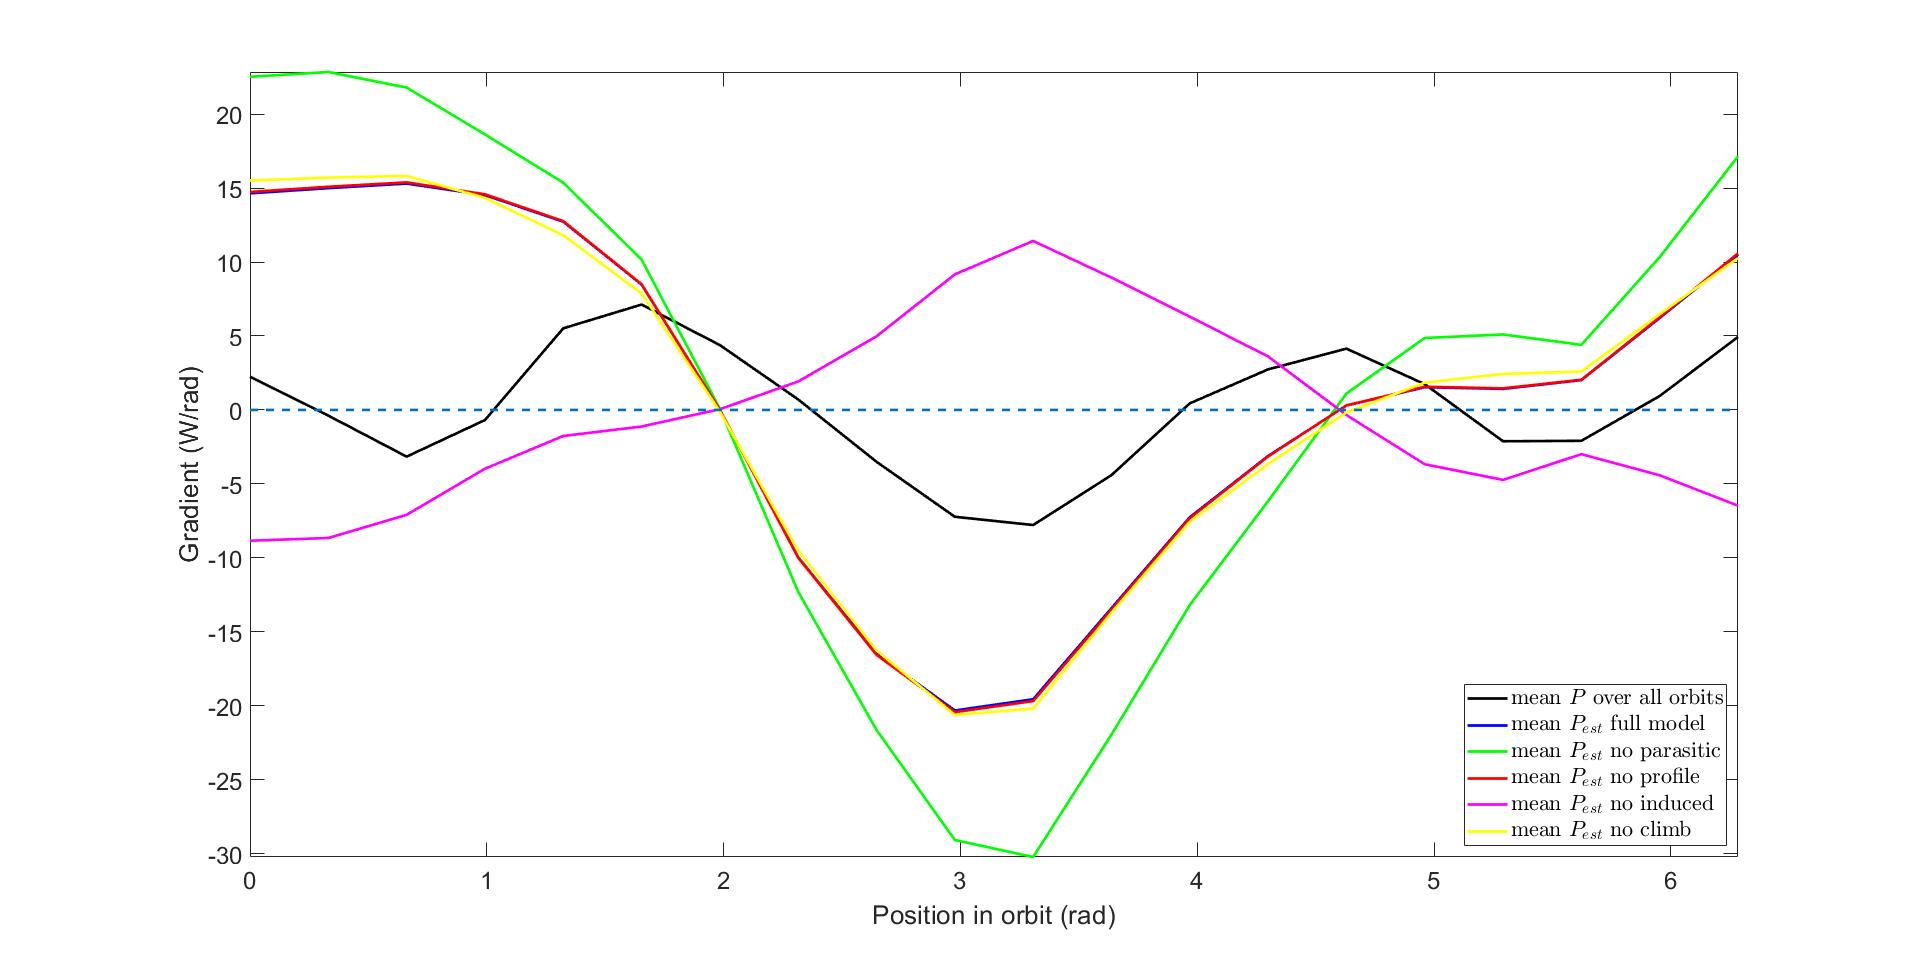
\includegraphics[width=0.5\textwidth, trim={6cm 0cm 4cm 2cm}, clip]{exp6Grad.jpg}
%	\caption{Here we see a direct comparison between our model's estimate and the dragless model's estimate for a single flight experiment along with the actual measured power onboard. This flight was 25 m radius orbit at an altitude of 25 m with a target linear velocity of 6 m/s in heavy wind conditions. The cyclical appearance of the power consumption corresponds to the wind heading relative to the quadrotor changing as it traverses the orbit. We can clearly see that neglecting drag when estimating power leads to underestimating the actual power considerably. Additionally, we can also see that the local minimas predicted by the dragless model occur further away from the true minima than our model's estimate.}
%\end{figure}
%
%\begin{figure}[tbp]
%	\centering
%	\label{fig:all8mps}
%	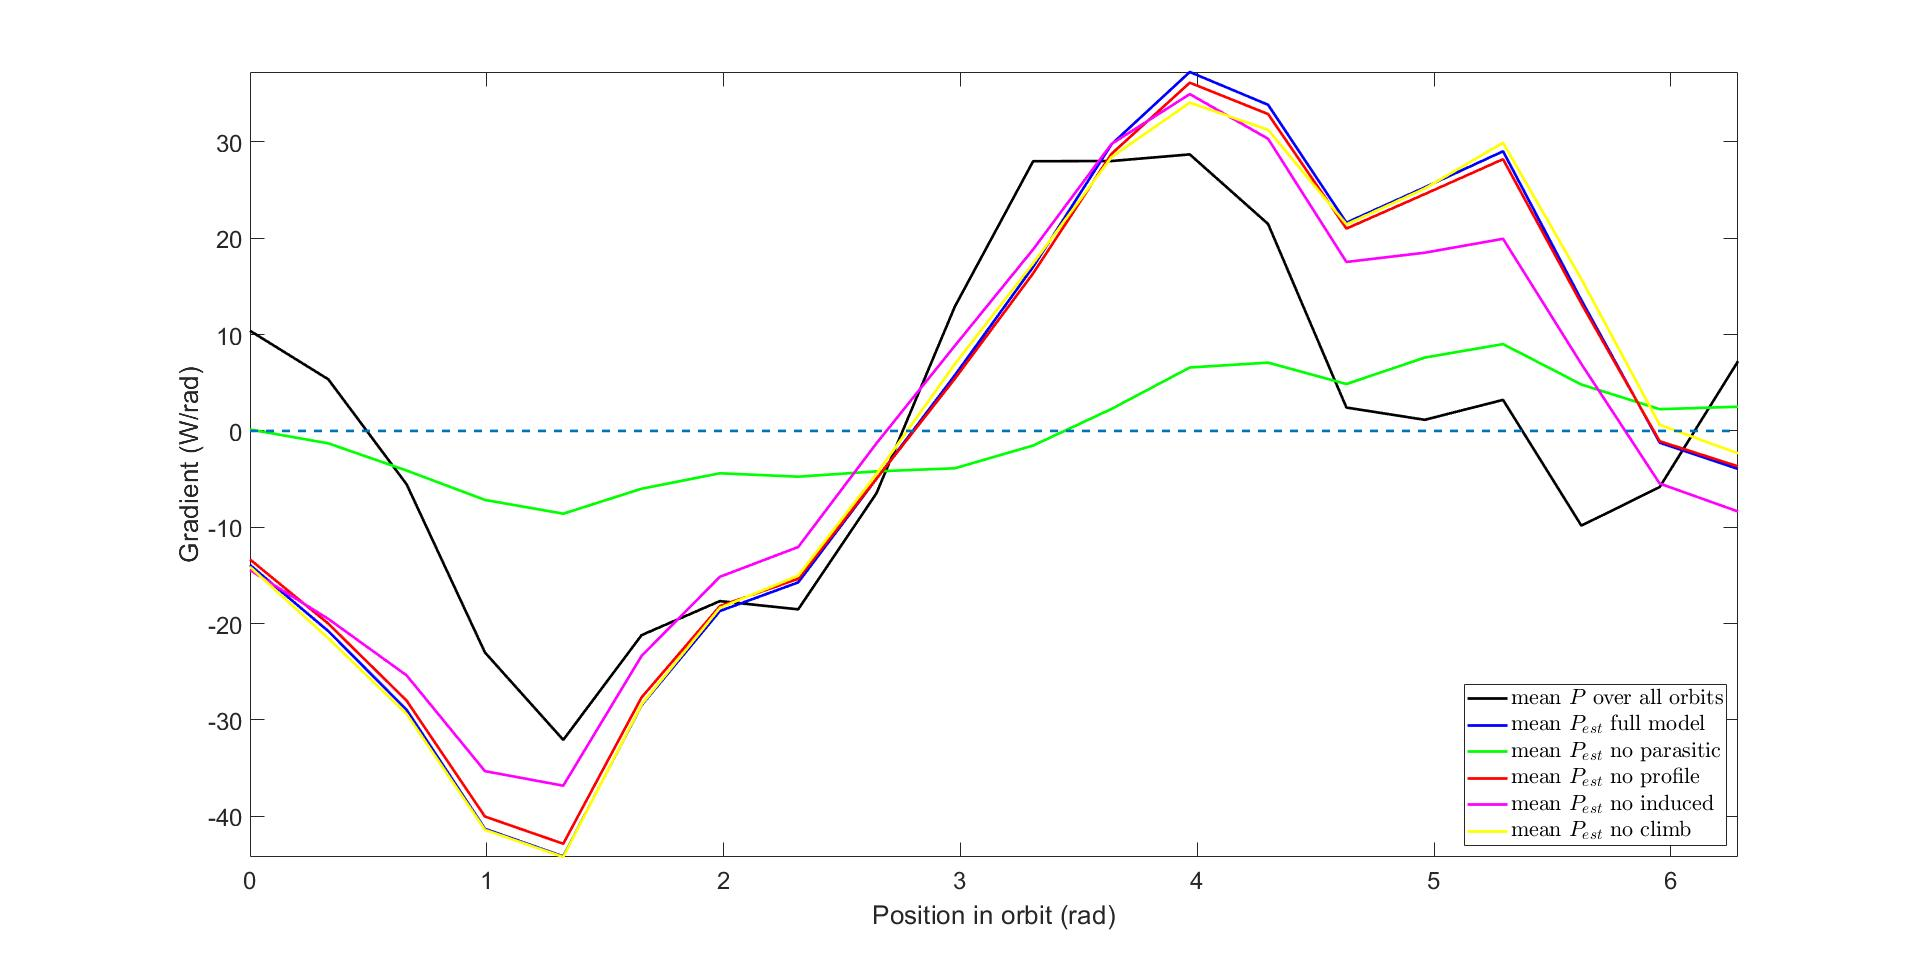
\includegraphics[width=0.5\textwidth, trim={6cm 0cm 4cm 2cm}, clip]{exp14Grad.jpg}
%	\caption{Comparing the mean of our model's predictions, the mean of the dragless model's predictions, and the measured power consumption for all 25 m orbits with an 8 $\frac{m}{s}$ linear velocity in heavy winds. Here the $0$ and $2\pi$ position correspond to the most northern point of the orbit and moving CCW around the orbit is positive. Because of the high amounts of additional drag being generated due to the high winds we see that the dragless model greatly underestimates power consumption and incorrectly predicts the location of minimum power.}
%\end{figure}


%\begin{table*}[ht]
%	\caption{$\hat{P}$ mean nRMSE (\%) and $\nabla \hat{P}$ mean RMSE (W/rad) for the removal of each term from the model}
%	\centering
%	\begin{tabular*}{0.63\textwidth}{cccccccccc}
%		\toprule
%		\textbf{Dropped} & \textbf{Hover} & \multicolumn{2}{c}{\textbf{2 m/s}} & \multicolumn{2}{c}{\textbf{4 m/s}} & \multicolumn{2}{c}{\textbf{6 m/s}} & \multicolumn{2}{c}{\textbf{8 m/s}} \\
%		\textbf{out term} & \textbf{$\hat{P}$} & \textbf{$\hat{P}$} & \textbf{$\nabla \hat{P}$} & \textbf{$\hat{P}$} & \textbf{$\nabla \hat{P}$} & \textbf{$\hat{P}$} & \textbf{$\nabla \hat{P}$} & \textbf{$\hat{P}$} & \textbf{$\nabla \hat{P}$} \\
%		\midrule
%		none        & 8.36     & 7.22   & 175.26 & 7.06   & 91.15   & 9.15   & 70.43 & 18.30 & 64.59 \\
%		$P_{par}$ & 13.57   & 11.20  & 189.70 & 12.65 & 93.65  & 15.99  & 70.61 & 18.26 & 59.60 \\
%		$P_{pro}$ & 20.97   & 17.89 & 175.39 & 17.51  & 91.08  & 13.28  & 70.17 & 11.36  & 64.02  \\
%		$P_{ind}$ & 80.70   & 81.86 & 167.41  & 78.12 & 95.20  & 68.44 & 73.34 & 54.73 & 63.57  \\
%		$P_{c}$    & 8.46     & 7.31   & 185.32 & 7.12   & 96.40  & 9.19   & 73.50 & 18.37  & 67.38 \\
%		\bottomrule 
%	\end{tabular*}
%	\label{tab:AblationRMSE}
%\end{table*}

\begin{table}[ht]
	\caption{$\hat{P}$ mean nRMSE (\%) for the removal of each term from the model}
	\centering
	\begin{tabular*}{0.4\textwidth}{cccccc}
		\toprule
		\textbf{Dropped} & \multirow{2}{*}{\textbf{Hover}} & \multirow{2}{*}{\textbf{2 m/s}} & \multirow{2}{*}{\textbf{4 m/s}} & \multirow{2}{*}{\textbf{6 m/s}} & \multirow{2}{*}{\textbf{8 m/s}} \\
		\textbf{out term} & & & & & \\
		\midrule
		none        & 8.36     & 7.22   & 7.06  & 9.15   & 18.30 \\
		$P_{par}$ & 13.57   & 11.20  & 12.65 & 15.99 & 18.26 \\
		$P_{pro}$ & 20.97   & 17.89 & 17.51 & 13.28  & 11.36 \\
		$P_{ind}$ & 80.70   & 81.86 & 78.12 & 68.44 & 54.73 \\
		$P_{c}$    & 8.46     & 7.31   & 7.12   & 9.19   & 18.37  \\
		\bottomrule 
	\end{tabular*}
	\label{tab:AblationRMSE}
\end{table}
